\documentclass{beamer}

\usepackage{paratype}
\setbeamerfont{frametitle}{family=\bf}

% Beamer theme settings
\usecolortheme{seagull}
\usenavigationsymbolstemplate{} % no navigation buttons

\usepackage[utf8]{inputenc}

\usepackage{graphicx}
\usepackage{epic}

\usepackage{amsmath}
\usepackage{amssymb}
\usepackage{amsthm}

\newcommand{\basetop}[1]{\vtop{\vskip-1ex\hbox{#1}}}
\newcommand{\source}[1]{\let\thefootnote\relax\footnotetext{\scriptsize\textcolor{kugray1}{Source: #1}}}

% for coloured code citation in text:
\usepackage{fancyvrb}

%%%%%%%%%%%%%%%%%%%%%%%%%%%%%%%%%
%%%%%    code sections   %%%%%%%%
%%%%%%%%%%%%%%%%%%%%%%%%%%%%%%%%%

% code highlighting commands in own block
\DefineVerbatimEnvironment{code}{Verbatim}{fontsize=\scriptsize}
\DefineVerbatimEnvironment{icode}{Verbatim}{fontsize=\scriptsize}

% Fancy code with color commands:
\DefineVerbatimEnvironment{colorcode}%
        {Verbatim}{fontsize=\scriptsize,commandchars=\\\{\}}

%%%%%%%%%%%%%%%%%%%%%%%%%%%%%%%%%%
%%%%%    some coloring    %%%%%%%%

\definecolor{Red}{RGB}{220,50,10}
\definecolor{Blue}{RGB}{0,51,102}
\definecolor{Yellow}{RGB}{102,51,0}
\definecolor{Orange}{RGB}{178,36,36}
\definecolor{Grey}{RGB}{180,180,180}
\definecolor{Green}{RGB}{20,120,20}
\definecolor{Purple}{RGB}{160,50,100}
\newcommand{\red}[1]{\textcolor{Red}{{#1}}}
\newcommand{\blue}[1]{\textcolor{Blue}{{#1}}}
\newcommand{\yellow}[1]{\textcolor{Yellow}{{#1}}}
\newcommand{\orange}[1]{\textcolor{Orange}{{#1}}}
\newcommand{\grey}[1]{\textcolor{Grey}{{#1}}}
\newcommand{\green}[1]{\textcolor{Green}{{#1}}}
\newcommand{\purple}[1]{\textcolor{Purple}{{#1}}}

% use "DIKU green" from our color theme for \emph
%\renewcommand{\emph}[1]{\textcolor{structure}{#1}}
\renewcommand{\emph}[1]{\textcolor{CosGreen}{ #1}}
% use some not-too-bright red for an \emp command
\definecolor{DikuRed}{RGB}{130,50,32}
\newcommand{\emp}[1]{\textcolor{DikuRed}{ #1}}
\definecolor{CosGreen}{RGB}{10,100,70}
\newcommand{\emphh}[1]{\textcolor{CosGreen}{ #1}}
\definecolor{CosBlue}{RGB}{55,111,122}
\newcommand{\emphb}[1]{\textcolor{CosBlue}{ #1}}
\definecolor{CosRed}{RGB}{253,1,1}
\newcommand{\empr}[1]{\textcolor{CosRed}{ #1}}

\newcommand{\mymath}[1]{$ #1 $}
\newcommand{\myindx}[1]{_{#1}}
\newcommand{\myindu}[1]{^{#1}}

\newtheorem{mydef}{Definition}
\newtheorem{mytheo}{Theorem}
\newtheorem{mylemma}{Lemma}

\title{OpenCL Day 3: Basic Block of Data-Parallel Programming and Applications}

\author{Cosmin Oancea and Troels Henriksen}

\date{February 4, 2019}

\begin{document}

\frame{\titlepage}

\section{Course Contents}

\begin{frame}
  \tableofcontents
\end{frame}

%%%%%%%%%%%%%%%%%%%%%%%%%%%%%%%%%%%%%%%%%%%%
%%% Reduction
%%%%%%%%%%%%%%%%%%%%%%%%%%%%%%%%%%%%%%%%%%%%

\section{Map and Reduce}

\subsection{Types, Semantics and Properties}

\begin{frame}[fragile,t]
   \frametitle{Basic Blocks of Parallel Programming: Map}

\bigskip

\emp{map} : $(\alpha \to \beta, [\alpha]) ~~\to~~ [\beta] $ has \emph{\em inherently parallel semantics}.
\smallskip

Applies a function to every element of the input array producing an array of equal length.

\bigskip

\begin{tabular}{crcccccl}
X = & \emph{map}(~f, ~ [& $a_1$, & $a_2$, & .., & $a_n$ & ])\\
    &      & $\downarrow$ & $\downarrow$ &  & $\downarrow$ & &\\
X $\equiv$ &  [  & \emph{f($a_1$)}, & \emph{f($a_2$)}, & .., & \emph{f($a_n$)} & ] &
\end{tabular}
\bigskip\pause

\emp{Map Fusion:} \emph{{\tt~~~map(f, map(g, A))} $~\equiv~$ {\tt map(f o g, A)}} \bigskip

\begin{tabular}{llllllll}
A & $\equiv$ & [ & $a_1$, & $a_2$, & $\ldots$, & $a_n$ & ] \\  
X = map(g, A) & $\equiv$ & [ & g($a_1$), &g($a_2$), &$\ldots$, &g($a_n$) &]\\
\emph{Y = map(f, X)} & $\equiv$ & [& \emph{f(g($a_1$))}, &\emph{f(g($a_2$))}, &$\ldots$, &\emph{f(g($a_n$))} &]\\
\emph{map(f o g, A)} & $\equiv$ & [& \emph{f(g($a_1$))}, &\emph{f(g($a_2$))}, &$\ldots$, &\emph{f(g($a_n$))} &]\\
\end{tabular}
\bigskip

Fusion is one of the most important optimizations, as it saves bandwidth!

\end{frame}


\begin{frame}[fragile,t]
   \frametitle{Basic Blocks of Parallel Programming: Reduce}

\bigskip

\emp{reduce} : $((\alpha, \alpha) \to \alpha),~ \alpha, [\alpha]) ~~\to~~ \alpha$

\smallskip

\emp{reduce}(~$\odot$, ~$0_\odot$, ~[$a_1$, $a_2$, ..., $a_n$]) $\equiv$ \emph{$0_\odot ~\odot ~a_1 ~\odot a_2 ~\odot ... \odot~ a_n$}

\smallskip

~~~~~where $\odot$ is an associative binary operator (\red{otherwise bug!})\\
~~~~~~~~~~~~~~~~$0_\odot$ is the neutral element of the monoid induced by $\odot$

\bigskip\pause

\begin{center} 
        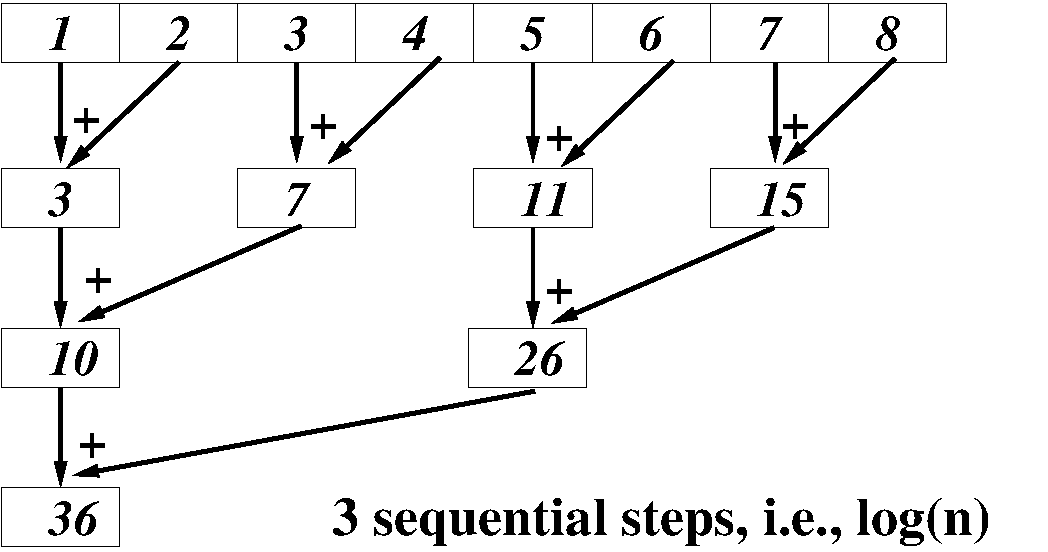
\includegraphics[height=20ex]{img/day3/ReduceEg.pdf} 
\end{center} 

Build programs by combining \emp{map}, \emp{reduce} and other such operators.

\end{frame}

\begin{frame}[fragile,t]
   \frametitle{Trivial Examples of Map-Reduce Programming}

\emp{Small Exercise:} write a function that receive as parameters a predicate 
$\texttt{p}~: ~ \alpha ~ \to ~ \texttt{bool}$ and an array {\tt A}, and that 
results in {\tt true} if all elements satisfy {\tt p} and in {\tt false} otherwise.\\\smallskip
\emp{Try to write (i) a divide-and-conquer and (ii) a map-reduce implementation.}
\medskip\pause

\begin{columns}
\column{0.4\textwidth}
\begin{colorcode}[fontsize=\small]
all(p, [ ])  = True
all(p, [x])  = p(x) 
all(p, x++y) = all(p, x) &&
               all(p, y)
\end{colorcode}
\column{0.58\textwidth}
\begin{colorcode}[fontsize=\small]
    all(p, x) = 
        y = map(p, x)
        z = reduce(&&, true, y)
        return z
\end{colorcode}
\end{columns}

\bigskip\pause
{\tt ++} denotes array concatenation.\smallskip

A well define divide and conquer implementation requires that any
split of the input array into {\tt x++y} gives the same result.\smallskip

(This is equivalent to the requirement that the binary operator of 
reduction is associative.)

\bigskip
Under this conditions, the two are equivalent: if you can write one, 
then you can derive the other (list homomorphic $\equiv$ map-reduce).

\end{frame}

\subsection{Efficient Sequentialization: Work, Depth, and Brent Lemma}

\begin{frame}[fragile,t]
   \frametitle{Asymptotic Work and Depth; Brent Lemma}

Assuming an infinity of processors:
\begin{itemize}
    \item \emp{Work Complexity $W(n)$}:       is the total \# of ops performed,\smallskip
    \item \emp{Depth/Step Complexity $D(n)$}: is the \# of sequential steps.\bigskip
    \item A parallel implem is {\bf work efficient} {\it iff} its work complexity
            is equal to the one of the golden sequential implem.\bigskip

    \item Work and Depth are good high-level approximations;
    \item If we know the work and depth asymptotic for a program,
            Brent Theorem offers good complexity bounds for a PRAM.
\end{itemize}

\begin{mytheo}[Brent Theorem]\label{BrentTh}
An algorithm of depth $D(n)$ and work $W(n)$ can be
simulated on a $P$-processor PRAM in time complexity T such that:\\\bigskip
\emp{$\ \ \ \ \ \ \ \ \ \ \ \ \ \ \ \ \frac{W(n)}{P} \leq T \leq \frac{W(n)}{P} + D(n)$}
\end{mytheo}

\end{frame}

\begin{frame}[fragile,t]
   \frametitle{Applying Brent Lemma to Map-Reduce Computation}

\begin{center} 
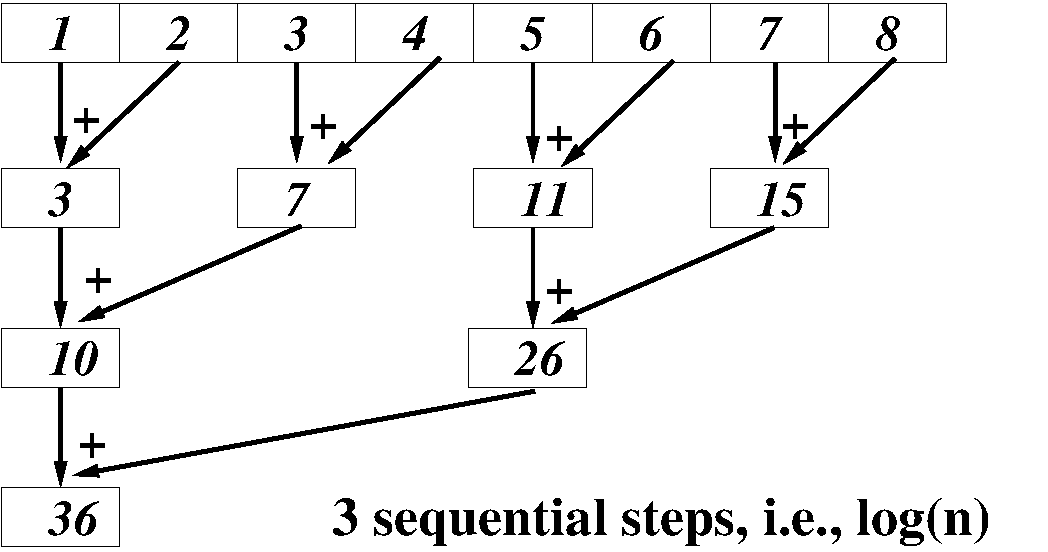
\includegraphics[height=20ex]{img/day3/ReduceEg.pdf} 
\end{center} 

Reducing an array of length {\tt n} with {\tt n/2} processors requires:
\begin{itemize}
    \item work $W(n) = n$ and 
    \item depth $D(n) = lg \ n$, i.e., number of sequential steps.
    \item Brent Theorem states the bounds for optimal runtime $T^{opt}$:\\\smallskip
            $ \frac{W(n)}{P} \leq T^{opt} \leq \frac{W(n)}{P} + D(n)$
\end  {itemize}

\end{frame}

\begin{frame}[fragile,t]
   \frametitle{Applying Brent Lemma to Map-Reduce Computation}

\begin{columns}
\column{0.37\textwidth}
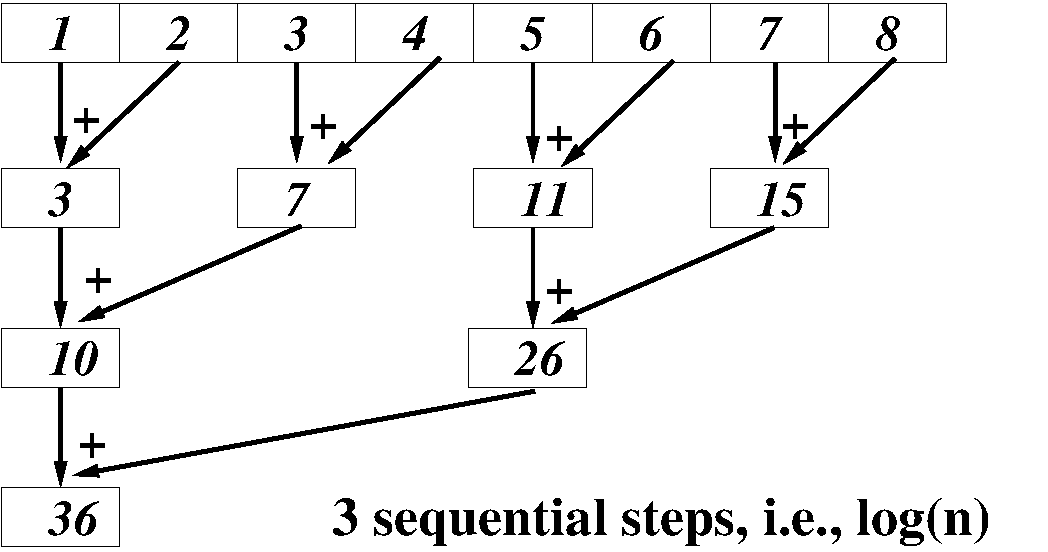
\includegraphics[height=13ex]{img/day3/ReduceEg.pdf} 
\column{0.61\textwidth}
Reducing an array of length {\tt n} with {\tt n/2} processors requires:
\begin{itemize}
    \item $W(n) = n$, $D(n) = lg \ n$.
    \item Optimal runtime $T^{opt}$ bounds:\\
            $ \frac{W(n)}{P} \leq T^{opt} \leq \frac{W(n)}{P} + D(n)$
\end  {itemize}
\end{columns}\bigskip

{\bf An optimized map-reduce computation can be implemented as:}
\begin{itemize}
    \item splits the input array into $P$ subarrays, each containing 
            about the same number of elements;\smallskip
    \item perform the computation sequentially on each subarray,
            but in parallel across subarrays;\smallskip
    \item reduce the $P$ per-processor results.
\end{itemize}\medskip
{\bf This leads to optimal runtime on $P$ processors:}\pause \emph{$O(\frac{n}{P} + lg \ P)$}
\bigskip

\emp{This kind of chunking is often referred to as:}\\
\emp{``efficient sequentialization of excess parallelism''!}

\end{frame}

%\begin{mytheo}[Optimized Map Reduce]\label{MapRed}
%Assume {\tt split$_p$} splits an array into $p$ subarrays, each containing about 
%the same number of elements. Denoting  
%$\mbox{~~~~~}{\tt redomap}~\odot ~ f ~ e_{\odot}~ X \equiv \ {\tt reduce}(~\odot,~ e_{\odot}, ~ {\tt map(f, X)~)}$\\
%the following equality holds:\\\smallskip
%
%\emp{${\tt redomap} \ \odot \ f \ e_{\odot} \ \ \equiv$}\\
%\emp{$\ \ \ \ \ \ \ \ \ \ \ \ \ \ \ \ \ \ \ ({\tt reduce} \ \odot \ e_{\odot}) \ \circ \ ({\tt map} \ ({\tt redomap} \ \odot \ f \ e_{\odot})) \ \circ \ {\tt split}_p$}
%\end{mytheo}


\subsection{Maximum Segment Sum Problem (MSSP)}

\begin{frame}[fragile,t]
  \frametitle{Almost Homomorphisms (Gorlatch)}

\emp{``Systematic Extraction and Implementation of Divide-and-Conquer Parallelism'', Sergei Gorlatch, 1996.} 
\bigskip

\emph{Intuition}: a non-homomorphic function $g$ can be sometimes lifted 
to a homomorphic one $f$, by computing a baggage of \emp{\em extra info}. 

\bigskip

The initial fun obtained by projecting the homomorphic result:\\
$g\mbox{ }=\pi~\circ~f$

\bigskip

\emp{\bf Maximum-Segment Sum Problem ({\sc mssp})}: \\
Given a list of integers, find the contiguous segment of the list 
whose members have the largest sum among all such segments.\\
The result is only the maximal sum (not the segment's members).
For simplicity lets assume we are interested only in {\bf positive sums}.

\bigskip

E.g., {\tt mss} [1, -2, 3, 4, -1, 5, -6, 1] = 11 \\
(the corresponding segment is [3, 4, -1, 5]). 

\end{frame}


\begin{frame}[fragile,t]
  \frametitle{Maximum Segment Sum (MSSP): Preliminary Reasoning}

\emp{\bf Maximum-Segment Sum Problem ({\sc mss})}: \\
Given a list of integers, find the contiguous segment of the list 
whose members have the largest sum among all such segments.\\
The result is only the maximal sum (not the segment's members).
For simplicity lets assume we are interested only in {\bf positive sums}.
\medskip

\red{A first straightforward/naive attempt:}
\begin{colorcode}
mss [ ]      = 0
mss [a]      = a \mymath{\uparrow} 0  \emp{//\mymath{\uparrow} denotes Max}
mss (x{\tt ++}\mbox{ }y) = mss(x) ??? mss(y)
\end{colorcode}

\bigskip
\bigskip

\begin{columns}
\column{0.58\textwidth}\pause
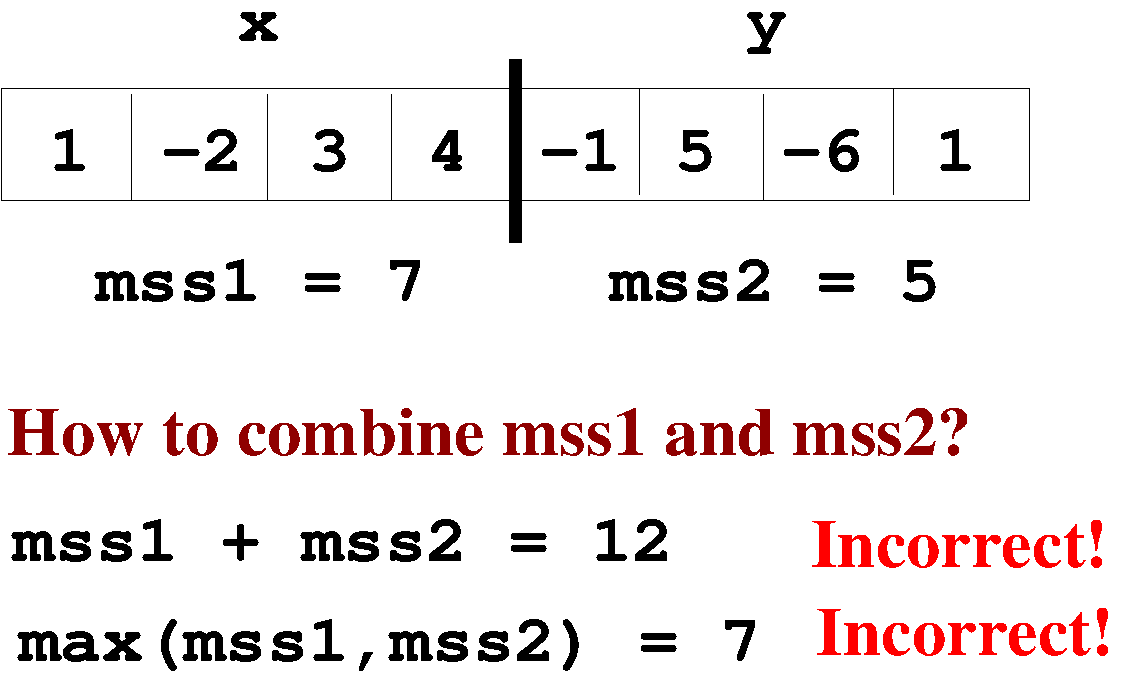
\includegraphics[height=20ex]{img/day3/mssp1}
\column{0.44\textwidth}
\red{Which case is problematic?}\pause\bigskip

\emph{Answer: when the segment of interest lies partly in {\tt x} and partly in {\tt y}!}
\end{columns}
\end{frame}

\begin{frame}[fragile,t]
  \frametitle{Maximum Segment Sum (MSSP): A Better Reasoning}

\red{The problematic case is when the segment of interest lies
     partly in {\tt x} and partly in {\tt y}!}
\bigskip

We need to compute extra information:\pause
\begin{itemize}
    \item maximum concluding segment
    \item maximum initial segment
    \item total segment sum
\end{itemize}\smallskip\pause

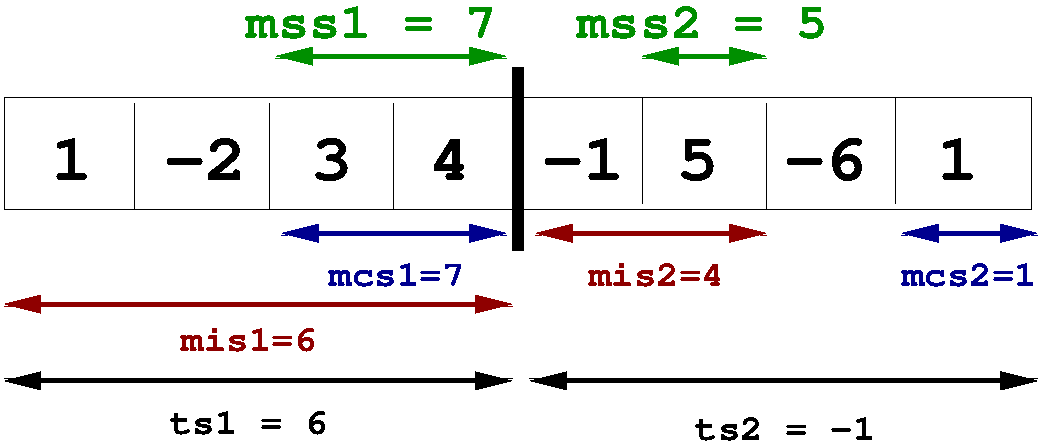
\includegraphics[height=22ex]{img/day3/mssp2}

\end{frame}

\begin{frame}[fragile,t]
  \frametitle{MSSP: Deriving the Implementation}

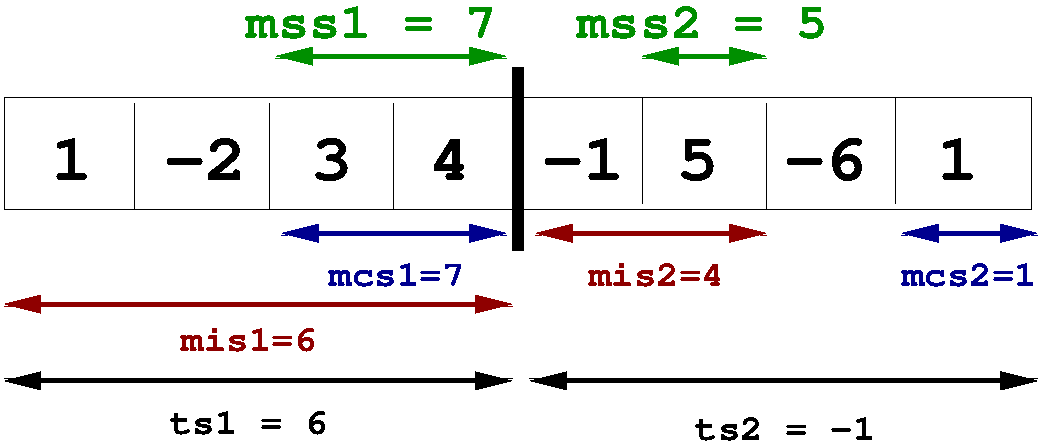
\includegraphics[height=22ex]{img/day3/mssp2}
\medskip
Lets compute the {\tt mis}, {\tt mcs}, {\tt mss}, and {\tt ts} for
the result of the two concatenating segments.

\bigskip
{\tt mis = \pause mis1 $\uparrow$ (ts1 + mis2)}
\medskip

{\tt mcs = \pause mcs2 $\uparrow$ (mcs1 + ts2)}
\medskip

{\tt mss = \pause mss1 $\uparrow$ mss2 $\uparrow$ (mcs1 + mis2)}
\medskip

{\tt ts~~= ts1 + ts2}
\end{frame}


\begin{frame}[fragile,t]
  \frametitle{MSSP: Map-Reduce C-ish Pseudocode}

\begin{columns}
\column{0.53\textwidth}
\begin{colorcode}
// x \mymath{\uparrow} y \mymath{\equiv} (x >= y) ? x : y
Qtup \blue{\mymath{\odot}} (Qtup x, Qtup y) \{
    Qtup r;
    r.mss = x.mss\mymath{\mbox{ }\uparrow\mbox{ }}y.mss\mymath{\mbox{ }\uparrow\mbox{ }}
            (x.mcs + y.mis);
    r.mis = x.mis\mymath{\mbox{ }\uparrow\mbox{ }}(x.ts + y.mis);
    r.mcs = (x.mcs + y.ts)\mymath{\mbox{ }\uparrow\mbox{ }}y.mcs;
    r.ts  = x.ts + y.ts;
    return r;
\}

Qtup \emp{f}(int x) \{
    Qtuple r;
    int x0 = x\mymath{\mbox{ }\uparrow\mbox{ }}0;
    r.mss = x0; r.mis = x0;
    r.mcs = x0; r.ts = x;
    return r;
\}
\end{colorcode}
\column{0.45\textwidth}
\begin{colorcode}
typedef struct msict \{
  int mss;
  int mis;
  int mcs;
  int ts;
\} Qtup;

int mss(int* xs) \{
    Qtup ne, res; 
    ne.mss = 0; ne.mis = 0;
    ne.mcs = 0; ne.ts  = 0;
    
    Qtup* ys = \emph{map}(\emp{f}, xs);
    res = \emph{reduce}(\blue{\mymath{\odot}}, ne, ys);
    return res.mss;
\}
\end{colorcode}
\end{columns}
\smallskip

The baggage: $3$ extra integers ({\tt misx, mcsx, tsx}) 
and a constant number of integer operations per communication stage. 
\medskip

\emp{For performance:} array {\tt ys} should not be manifested in memory;\\
fuse the {\tt map} with the {\tt reduce} operations.

\end{frame}

\subsection{Exercise 1: OpenCL Implementation of MSSP}

\begin{frame}[fragile,t]
  \frametitle{Exercise 1: OpenCL Implementation of MSSP}

Troels should add description here of what does he want the students to do!
\end{frame}

%%%%%%%%%%%%%%%%%%%%%%%%%%%%%%%%%%%%%%%%%
%%% SCAN
%%%%%%%%%%%%%%%%%%%%%%%%%%%%%%%%%%%%%%%%%
\section{Scan and Applications}

\begin{frame}
  \tableofcontents[currentsection]
\end{frame}

\subsection{Scan: Type, Semantics, Asymptotic, Parallel Implementation}

\begin{frame}[fragile,t]
  \frametitle{Scan: A Basic Block of Data-Parallel Programming}

Scan is also known as parallel prefix sum:
\begin{itemize}
\item computes all partial prefixes of an array;
\item similar type with reduce, except that it returns an array;\medskip
\item \emp{exclusive scan}: result array starts with the neutral element;
\item \emph{inclusive scan}: starts with the first element of the input array;\medskip
\item Inclusive scan is slightly more useful than exclusive scan.
\end{itemize}\bigskip\pause

\emp{{\tt scan$^{exc}$: ( ($\alpha$,$\alpha$)$\rightarrow\alpha$),$~\alpha$, [n]$\alpha$ )$~\rightarrow~$[n]$\alpha$}}\\
        \emph{\tt scan$^{exc}(\odot$,e,[x$_1$,$\ldots$,x$_n$])~=~[e,e$\odot$x$_1$,$\ldots$,e$\odot$x$_1\odot\ldots$x$_{n-1}$]}\\
        i.e., \emp{{\tt{}e:$\alpha$, x$_i$:$\alpha,~\forall i$}}, and 
        \emp{\tt~~~$\odot$:$(\alpha,\alpha)\rightarrow\alpha$}.\bigskip

\emp{{\tt scan$^{inc}$: ( ($\alpha$,$\alpha$)$\rightarrow\alpha$),$~\alpha$, [n]$\alpha$ )$~\rightarrow~$[n]$\alpha$}}\\
        \emph{\tt scan$^{inc}(\odot$,e,[x$_1$,$\ldots$,x$_n$])~=~[x$_1$,~x$_1$$\odot$x$_2$,$\ldots$,x$_1\odot\ldots\odot$x$_{n}$]}\\
        i.e., \emp{{\tt{}e:$\alpha$, x$_i$:$\alpha,~\forall i$}}, and 
        \emp{\tt~~~$\odot$:$(\alpha,\alpha)\rightarrow\alpha$}.

\end{frame}

\begin{frame}[fragile,t]
  \frametitle{Parallel Exclusive Scan with Associative Operator $\oplus$}
\bigskip

\begin{columns}
\column{0.4\textwidth}
        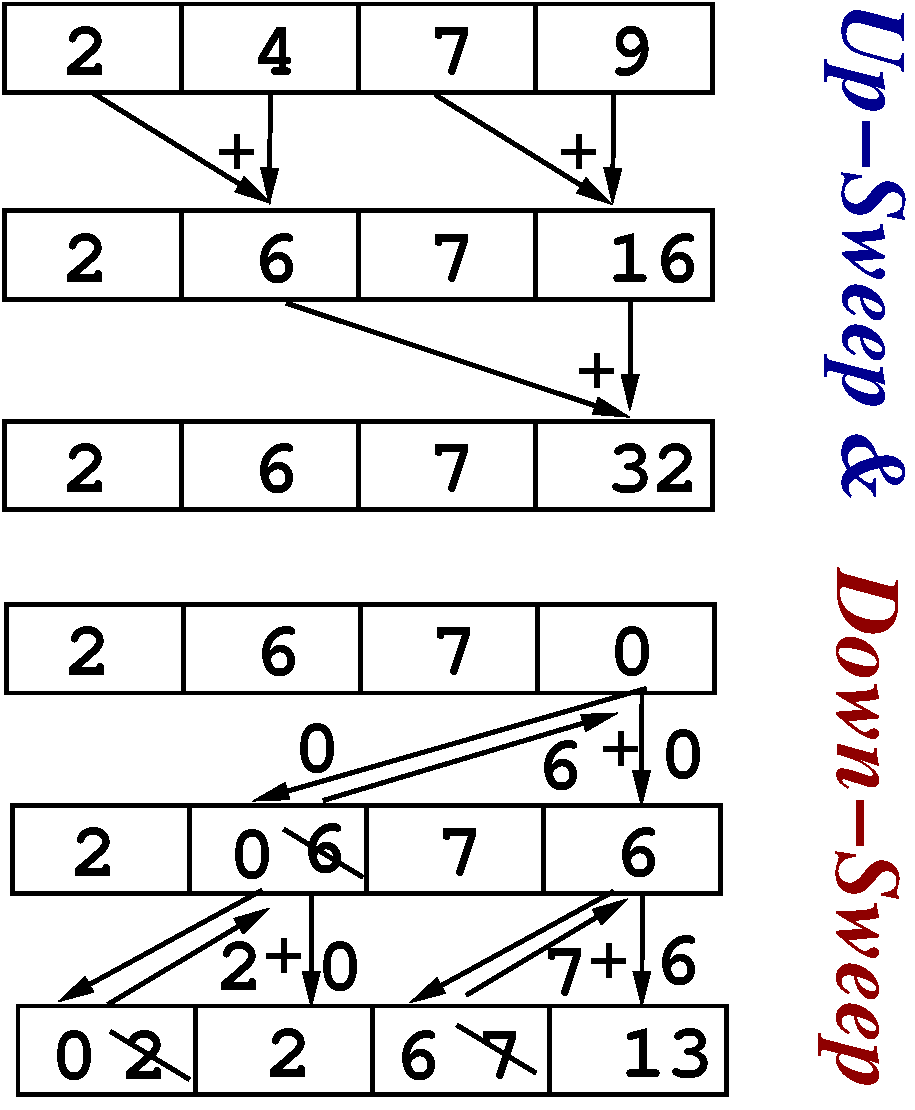
\includegraphics[height=30ex]{img/day3/ScanEg} 
\column{0.6\textwidth}
Two Steps:
\begin{itemize}
    \item \blue{Up-Sweep:} similar with reduction
    \item Root is replaced with neutral element.
    \item \emp{Down-Sweep:} 
    \begin{itemize}
        \item the left child sends its value to parent and 
                updates its value to that of parent.
        \item the right-child value is given by $\oplus$ 
                applied to the left-child value and
                the (old) value of parent.
        \item note that the right child is in fact the parent,
                i.e., in-place algorithm.
    \end  {itemize}
\end  {itemize}
\end{columns}\bigskip

{\bf Scan's Work and Depth:} \emph{$D(n) = \Theta(lg \ n), W(n) = \Theta(n)$}

\end{frame}

\begin{frame}[fragile,t]
  \frametitle{Wavefront-Level Inclusive Scan for GPUs}

\begin{columns}
\column{0.46\textwidth}
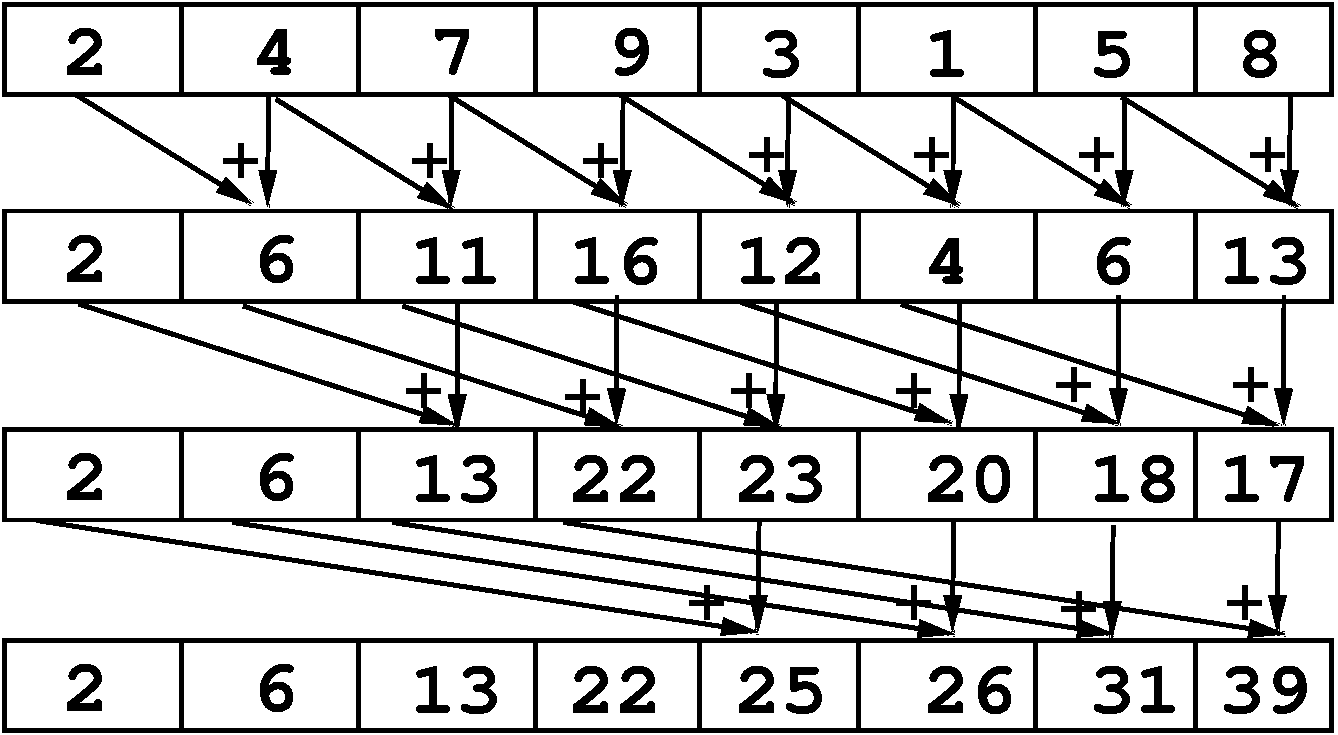
\includegraphics[height=15ex]{img/day3/incScanGPU} 
\column{0.53\textwidth}
\begin{colorcode}
Input:  array A of n=\mymath{2\myindu{k}} elements
                       of type \mymath{\alpha}
        \mymath{\oplus} : \mymath{(\alpha,\alpha)\to\alpha} associative
Output: B = [a\mymath{\myindx{1}}, a\mymath{\myindx{1}}\mymath{\oplus}a\mymath{\myindx{2}}, \mymath{\ldots} ,\mymath{\oplus\myindx{j=0}\myindu{n-1}} a\mymath{\myindx{j}}]
1.  forall i = 0 : n-1 do
2.    B[i] \mymath{\leftarrow} A[i]
3.  endfor
4.  for d = 0 to k-1 do
5.    h = 2\mymath{\myindu{d}}
6.    forall i = h to n-1 do 
7.      B[i] \mymath{\leftarrow} B[i-h] \mymath{\oplus} B[i]
8.    endfor
9.  endfor
\end{colorcode}
\end{columns}\bigskip

\emp{Offers better performance because it operates in one sweep rather than two!}

\end{frame}

\subsection{Exercise 2: Intra-Wave Scan Implementation}

\begin{frame}[fragile,t]
  \frametitle{Exercise 2: Intra-Wave Scan Implementation}

\begin{columns}
\column{0.46\textwidth}
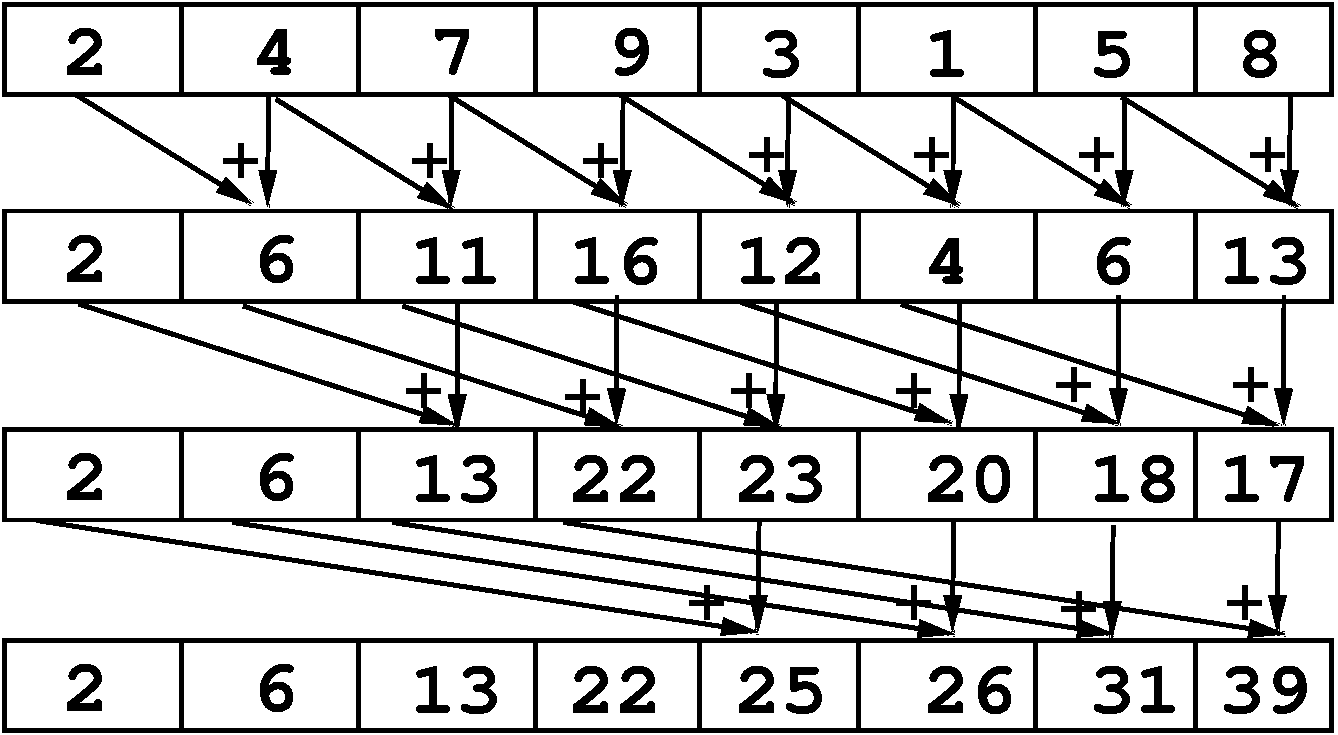
\includegraphics[height=15ex]{img/day3/incScanGPU} 
\column{0.53\textwidth}
\begin{colorcode}
Input:  array A of n=\mymath{2\myindu{k}} elements
                       of type \mymath{\alpha}
        \mymath{\oplus} : \mymath{(\alpha,\alpha)\to\alpha} associative
Output: B = [a\mymath{\myindx{1}}, a\mymath{\myindx{1}}\mymath{\oplus}a\mymath{\myindx{2}}, \mymath{\ldots} ,\mymath{\oplus\myindx{j=0}\myindu{n-1}} a\mymath{\myindx{j}}]
1.  forall i = 0 : n-1 do
2.    B[i] \mymath{\leftarrow} A[i]
3.  endfor
4.  for d = 0 to k-1 do
5.    h = 2\mymath{\myindu{d}}
6.    forall i = h to n-1 do 
7.      B[i] \mymath{\leftarrow} B[i-h] \mymath{\oplus} B[i]
8.    endfor
9.  endfor
\end{colorcode}
\end{columns}

\begin{itemize}
    \item TODO: Cosmin should write exercise description here!!!
\end{itemize}

\end{frame}

\subsection{Other Data-Parallel Operators: Scatter, Partition}

\begin{frame}[fragile,t]
  \frametitle{Scatter: Parallel Write Operator}

{\bf Scatter} \emph{updates in parallel and in place} an input array with a set of values at specified indices:
\smallskip

\emph{scatter : ([m]$\alpha$, [n]int, [n]$\alpha$) $\rightarrow$ [m]$\alpha$}
\bigskip

A (data vector)    {\tt~=[b0, b1, b2, b3]}\\
I (index vector)   {\tt~=[2,~~4,~~1,~~-1]}\\
X (input array)    {\tt~=[a0,~a1,~a2,~a3,~a4,~a5]}\\
\emp{scatter X I A {\tt~~~=[a0,~b2,~b0,~a3,~b1,~a5]}}
\bigskip\pause

\emph{scatter} has $D(n)=\Theta(1)$ and $W(n)=\Theta(n)$,\\
i.e., requires {\tt n} update operations ({\tt n} is the size of I or A, not of X!).\bigskip

\end{frame}

\begin{frame}[fragile,t]
  \frametitle{Exercise 3: Partition2 Operator}

{\bf Type and Semantics of Partition2}:\\
\emph{\tt partition2 : ($\alpha\rightarrow$Bool, [n]$\alpha$) $\rightarrow$ (int,[n]$\alpha$)}\\\bigskip

Partition2 receives as input a predicate and an array and results in:
\begin{itemize}
    \item an integer denoting the number of elements that succeed under predicate, tupled with
    \item a new array, having the same elements as the input array, but reordered
            such as the elements that succeed under the predicate occur before the others.
    \item The partial order of the elements that succeed/fail should be respected.
\end{itemize}\bigskip

\begin{colorcode}
bool odd(int v) \{ return (bool)(v & 1); \}
partition2( odd, [5, 4, 2, 10, 3, 7, 8] ) should result in
             (3, [5, 3, 7, 4, 2, 10, 8])
\end{colorcode}

\end{frame}

\begin{frame}[fragile,t]
  \frametitle{Exercise 3, Step 1: Partition2 High-Level Implementation}

\begin{colorcode}
bool odd(int v) \{ return (bool)(v & 1); \}
partition2( odd, [5, 4, 2, 10, 3, 7, 8] ) should result in
             (3, [5, 3, 7, 4, 2, 10, 8])
\end{colorcode}

Step 1: implement partition2 based on map, scan and scatter (?)\pause

TODO: Cosmin needs to write the implementation in a more imperative style!

\begin{columns}
\column{0.59\textwidth}
\begin{colorcode}
let partition2 [n] (X : [n]i32) : 
              ([n]i32, [n]i32) =
 let cs = map cond X
 let tfs= map (\mymath{\lambda}f->if f then 1 
                        else 0) cs
 let isT= scan (+) 0 tfs
 let i  = isT[n-1]

 let ffs= map (\mymath{\lambda}f->if f then 0 
                        else 1) cs
 let isF= map (+i) (scan (+) 0 ffs)
 let inds=map (\mymath{\lambda}(c,iT,iF) -> 
                  if c then iT-1 
                       else iF-1
              ) (zip cs isT isF)
 let res = scatter (scratch n) inds X
 in (i, res)
\end{colorcode}
\column{0.4\textwidth}\vspace{-2ex}
\begin{colorcode}[fontsize=\scriptsize]
Assume X = [5,4,2,3,7,8], and 
cond is T(rue) for even nums.\pause
n   = 6
cs  = [F, T, T, F, F, T]
tfs = [0, 1, 1, 0, 0, 1]

isT = [0, 1, 2, 2, 2, 3]
i   = 3

ffs = [1, 0, 0, 1, 1, 0]
isF = [4, 4, 4, 5, 6, 6]

inds= [3, 0, 1, 4, 5, 2]


flags  = [3, 0, 0, 3, 0, 0]
Result = [4, 2, 8, 5, 3, 7] 
\end{colorcode}
\end{columns}


\end{frame}


\subsection{Exercise 3, Step 2: Partition2 OpenCL Implementation}

\begin{frame}[fragile,t]
  \frametitle{Exercise 3: Implement Partition2 in OpenCL}

\begin{itemize}
    \item TODO: Cosmin should write the exercise description here!!!
\end{itemize}

\end{frame}

\section{Segmented Scan and Applications}

\subsection{Segmented Scan: Type, Semantics, Asymptotic, Impleme}

\begin{frame}[fragile,t]
  \frametitle{What is a Segmented Scan?}

\pause
Assume an \emp{irregular} matrix (two-dimensional array), 
i.e., rows have different number of elements.\medskip

{\bf Segmented Scan Intuition}: the operation that scans each
row of an irregular matrix and returns the result.\medskip

{\bf Flat Representation of a 2D irregular array:} flag + value arrays:
\pause
\begin{columns}
\column{0.33\textwidth}
\begin{colorcode}
[ [1, 2, 3]
, [4, 5, 6, 7, 8]
, [9, 10]
]
\end{colorcode}
\column{0.58\textwidth}
\begin{colorcode}
Flag Array:
[1, 0, 0, 1, 0, 0, 0, 0, 1, 0 ]
Value Array:
[1, 2, 3, 4, 5, 6, 7, 8, 9, 10]
\end{colorcode}
\end{columns}\medskip

\emp{The flag array} marks with one (or something different than zero) 
the start of a row/segment, the other elements are zero.\medskip

\emp{The value array}: flat sequence of elements. \bigskip

\begin{scriptsize}
\emp{{\tt sgmScan$^{inc/exc}$:~(($\alpha$,$\alpha$)$\rightarrow\alpha$),$~\alpha$,~[n]int,~[n]$\alpha$)$~\rightarrow~$[n]$\alpha$}}\\
\begin{colorcode}
\emp{sgmScan\mymath{\myindu{inc}}((+), 0, [1, 0, 0, 1, 0, 0,  0,  0,  1, 0 ]}
               \emp{ , [1, 2, 3, 4, 5, 6,  7,  8,  9, 10])} \mymath{\equiv}\pause
               \emph{   [1, 3, 6, 4, 9, 15, 22, 30, 9, 19]}
\end{colorcode}
\end{scriptsize}
\end{frame}

\begin{frame}[fragile,t]
  \frametitle{Intuition: How Does the Implementation Looks Like?}

Slide taken from CMU 15-418: Parallel Computer Architecture and Programming (Spring 2012).
Segmented Exclusive Scan:\vspace{-2ex}

\begin{center}
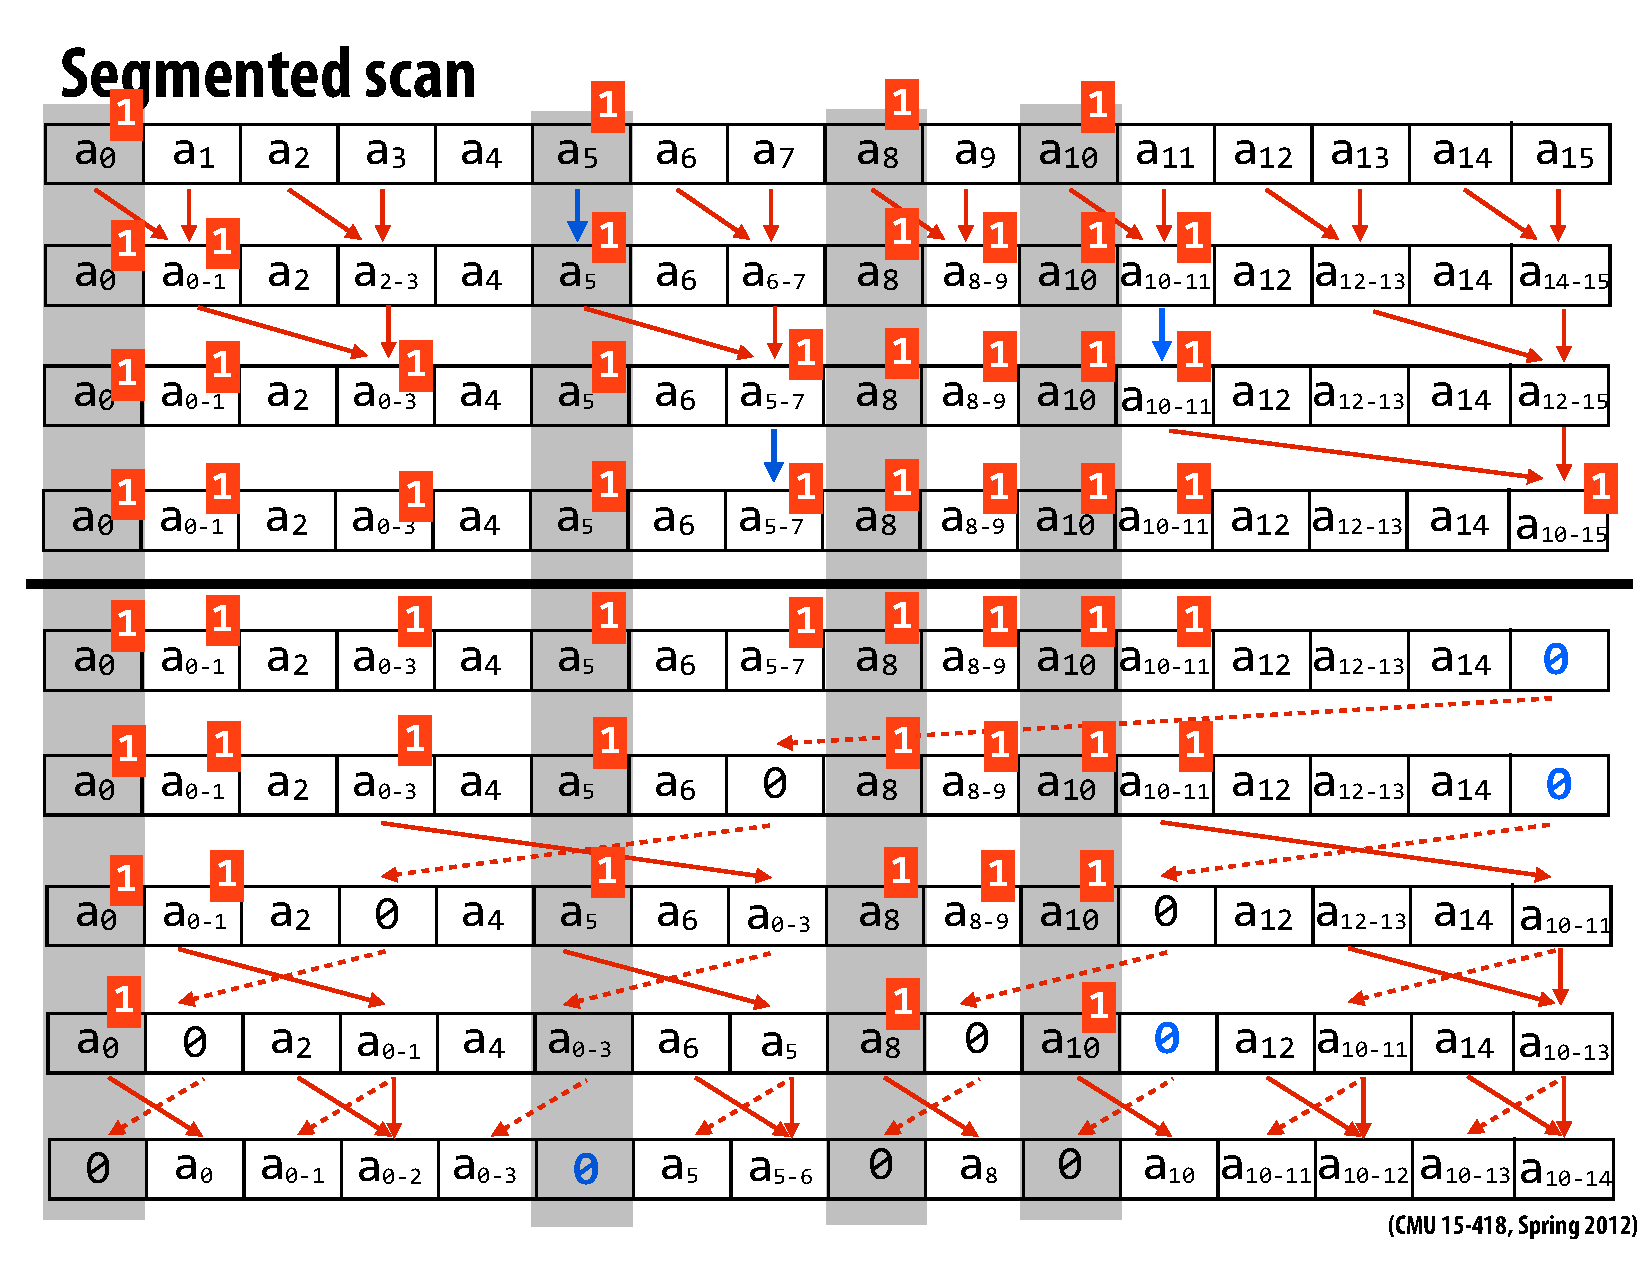
\includegraphics[height=42ex]{img/day3/SgmExcScanFig} 
\end  {center}
\end{frame}

\begin{frame}[fragile,t]
  \frametitle{Segmented Exclusive Scan Algorithm And Complexity}
\vspace{-1ex}
\begin{columns}
\column{0.31\textwidth}
\begin{itemize} 
    \item While there will be more branches, the asymptotic
            is the same as the one for reduce and scan:
    \item \emph{$D(n) = \Theta(lg \ n)$},\\\emp{$W(n) = \Theta(n)$!}
    \item That's the good news!
    \item The bad news:
\end{itemize}\pause
\column{0.75\textwidth}
\begin{colorcode}[fontsize=\scriptsize]
Input:  flag array F of n=2\mymath{\myindu{k}} of ints
        data array A of n=2\mymath{\myindu{k}} elems of type T
        \mymath{\oplus::T\times T\rightarrow T} associative
Output: B = segmented scan of 2-dim array A
1.  \emph{FORALL i = 0 to n-1 do} B[i] \mymath{\leftarrow} A[i] \emph{ENDDO}
2.  \emp{FOR d = 0 to k-1 DO} \emph{// up-sweep}
3.    \emph{FORALL i = 0 to n-1 by 2\mymath{\myindu{d+1}} DO} 
4.      IF F[i+2\mymath{\myindu{d+1}}-1] == 0 THEN 
5.          B[i+2\mymath{\myindu{d+1}}-1] \mymath{\leftarrow} B[i+2\mymath{\myindu{d}}-1] \mymath{\oplus} B[i+2\mymath{\myindu{d+1}}-1]
6.      ENDIF
7.      F[i+2\mymath{\myindu{d+1}}-1] \mymath{\leftarrow} F[i+2\mymath{\myindu{d}}-1] .|. F[i+2\mymath{\myindu{d+1}}-1]
8.  \emp{ENDDO} \emph{ENDDO}
9.  B[n-1] \mymath{\leftarrow} 0
10. \emp{FOR d = k-1 downto 0 DO} \emph{// down-sweep}
11.   \emph{FORALL i = 0 to n-1 by 2\mymath{\myindu{d+1}} DO} 
12.     tmp \mymath{\leftarrow} B[i+2\mymath{\myindu{d}}-1]
13.     IF \alert{F\_original}[i+2\mymath{\myindu{d}}] \mymath{\neq} 0 THEN
14.          B[i+2\mymath{\myindu{d+1}}-1] \mymath{\leftarrow} 0
15.     ELSE IF F[i+2\mymath{\myindu{d}}-1] \mymath{\neq} 0 THEN
16.          B[i+2\mymath{\myindu{d+1}}-1] \mymath{\leftarrow} tmp
17.     ELSE B[i+2\mymath{\myindu{d+1}}-1] \mymath{\leftarrow} tmp \mymath{\oplus} B[i+2\mymath{\myindu{d+1}}-1]
18.     ENDIF
19.     F[i+2\mymath{\myindu{d+1}}-1] \mymath{\leftarrow} 0
20. \emp{ENDDO} \emph{ENDDO}
\end{colorcode}
\end{columns}

\end{frame}

\begin{frame}[fragile,t]
  \frametitle{Segmented Inclusive Scan is a Sort of Scan!}
\pause

Can be implemented as a scan with a modified binary-associative
operator that operates on boolean-value (or int-value) tuples. 
\bigskip

We need to define {\tt zip} first, which performs SoA to AoS transform:\\\smallskip
\begin{scriptsize}
\emp{{\tt zip: ( [n]$\alpha$, [n]$\beta$ )$~\rightarrow~$[n]$(\alpha,\beta)$}}\\
\emph{\tt zip([x$_1$,$\ldots$,x$_n$], [y$_1$,$\ldots$,y$_n$])~=~[(x$_1$,y$_1$),$\ldots$,(x$_{n}$,y$_{n}$)]}\\\medskip
\end{scriptsize}
\medskip\pause

\begin{colorcode}[fontsize=\scriptsize]
typedef Tuple \{
    \mymath{\alpha}    val;
    bool flg;
\} Tup;

Tup \mymath{\odot\myindu{sgm}}(Tup x, Tup y) \{
    Tup r;
    r.flg = x.flg || y.flg;
    r.val = y.flg ? y.val : x.val \mymath{\odot} y.val;
    return r;
\}

\mymath{\alpha}* sgmScan\mymath{\myindu{inc}} (\mymath{\odot: (\alpha,\alpha)\to\alpha}, \mymath{\alpha} ne, \mymath{\alpha}* flags, \mymath{\alpha}* vals) \{
    Tup nes; nes.flg = false; nes.val = ne;
    Tup* X = zip(flags, vals);
    return scan\mymath{\myindu{inc}}(\mymath{\odot\myindu{sgm}}, nes, X)
\}
\end{colorcode}

\end{frame}



\subsection{Application: Sparse Matrix-Vector Multiplication}

\begin{frame}[fragile,t]
  \frametitle{Sparse Matrix-Vector Multiplication}

TODO: COSMIN should continue here!!!

\end{frame}

\subsection{Exercise 4: Sparse Matrix-Vector Mult in OpenCL}

\begin{frame}[fragile,t]
  \frametitle{Exercise 4: Sparse Matrix-Vector Mult in OpenCL}

TODO: COSMIN should continue here!!!

\end{frame}


\end{document}
